%%   (set-keyboard-coding-system 'utf-8)
\documentclass[tikz]{standalone}
\usepackage{tikz}
\usepackage{pgfplots}
\usetikzlibrary{matrix, positioning, shapes}
\usetikzlibrary{arrows, arrows.meta, automata, shadows, patterns}
\usetikzlibrary{calc, decorations.pathmorphing}

\pgfdeclaredecoration{penciline}{initial}{
  \state{initial}[width=+\pgfdecoratedinputsegmentremainingdistance,
  auto corner on length=1mm,]{
    \pgfpathcurveto%
    {% From
      \pgfqpoint{\pgfdecoratedinputsegmentremainingdistance}
      {\pgfdecorationsegmentamplitude}
    }
    {%  Control 1
      \pgfmathrand
      \pgfpointadd{\pgfqpoint{\pgfdecoratedinputsegmentremainingdistance}{0pt}}
      {\pgfqpoint{-\pgfdecorationsegmentaspect
          \pgfdecoratedinputsegmentremainingdistance}%
        {\pgfmathresult\pgfdecorationsegmentamplitude}
      }
    }
    {%TO 
      \pgfpointadd{\pgfpointdecoratedinputsegmentlast}{\pgfpoint{1pt}{1pt}}
    }
  }
  \state{final}{}
}

\begin{document}
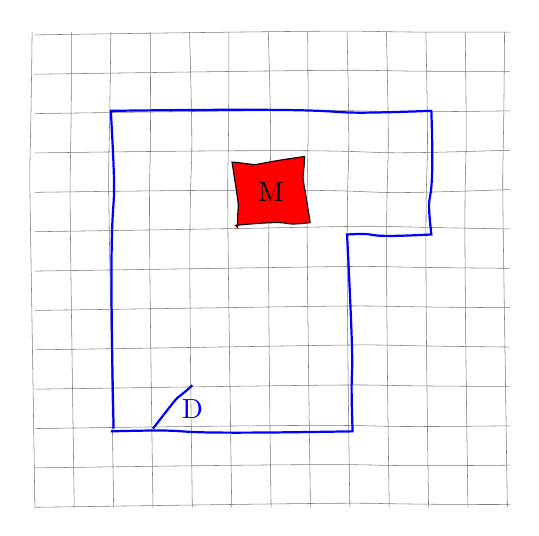
\begin{tikzpicture}[decoration=penciline, decorate]
  \draw[decorate,style=help lines] (-1,-1) grid[step=0.5cm] (5,5);
  \draw[decorate,thick,blue] (0,0) -- (0,4) -- (4,4) -- (4,2.5) -- (3,2.5) -- (3,0) -- (0,0);
  \draw[decorate,thick,blue] (0.5,0) -- (1,0.5) node[below] {D};
  \node[decorate,draw,inner sep=0.3cm,fill=red] (machine) at (2,3) {M};

  %\draw[decorate,ultra thick,blue] (3,3) arc (0:-90:2cm);
        % supposed to be an arc
  %\draw[decorate,thick,pattern=north east lines] (-0.4cm,-0.8cm) rectangle (1.2,-2);
  %\node[decorate,draw,inner sep=0.5cm,fill=yellow,circle] (a) at (2,0) {};
  % That's not even an ellipse
  %\node[decorate,draw,inner sep=0.3cm,fill=red] (b) at (2,-2) {};
  %\draw[decorate] (b) to[in=-45,out=45] (a);
        % This was supposed to be an edge
  %\node[decorate,draw,minimum height=2cm,minimum width=1cm] (c) at (-1.5,0) {};
  %\draw[decorate,->,dashed] (-0.5cm,-0.5cm) -- (-0.5cm,3.5cm)  -| (c.north);
\end{tikzpicture}

\end{document}